\section{Linux render-stack}


\begin{figure}[H] \label{render-stack}
    \caption{Drivers: everything on the right of a driver is hardware-agnostic, everything on the left hardware-specific. Note that Xorg and mesa don't use the same drivers. 
    Historically, linux used to only do 2d-graphics. For a brief time after 3d-cards arrived, OpenGl instructions were passed through Xorg. Only later was mesa allowed to bypass Xorg - 
    hence the name \emph{direct} rendering infrastructure.}
    \centering
    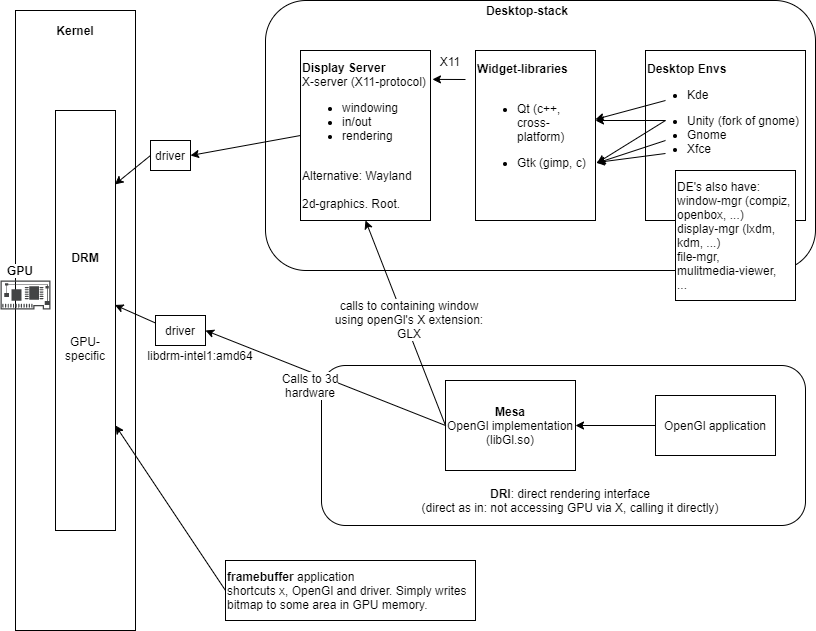
\includegraphics[width=0.8\linewidth]{images/render-stack.png}
\end{figure}


